\documentclass[11pt]{beamer}

%%%%%%%% tema %%%%%%%%
\mode<presentation> {
\usetheme{Singapore}
%\usecolortheme{albatross}
}

\usepackage[spanish]{babel}
\usepackage[utf8]{inputenc}
\usepackage{graphicx} 
\usepackage{booktabs}
\usepackage{listings} %Inserta código en el archivo
\usepackage{hyperref} %permite insertar direcciones web

\usepackage{color}
 
\definecolor{codegreen}{rgb}{0,0.6,0}
\definecolor{codegray}{rgb}{0.5,0.5,0.5}
\definecolor{codepurple}{rgb}{0.58,0,0.82}
\definecolor{backcolour}{rgb}{0.95,0.95,0.92}


\lstdefinestyle{mystyle}{
    backgroundcolor=\color{backcolour},   
    commentstyle=\color{codegreen},
    keywordstyle=\color{magenta},
    numberstyle=\tiny\color{codegray},
    stringstyle=\color{codepurple},
    basicstyle=\footnotesize,
    breakatwhitespace=false,         
    breaklines=true,                 
    captionpos=b,                    
    keepspaces=true,                 
    numbers=left,                    
    numbersep=5pt,                  
    showspaces=false,                
    showstringspaces=false,
    showtabs=false,                  
    tabsize=2
}
 
\lstset{style=mystyle}






\institute[INS] 
{
%================= logos no meio =====================
\vspace*{-0.35cm}

\includegraphics[width=1.8cm]{img/ImagenN03.png}
\hspace*{0.25cm}~%
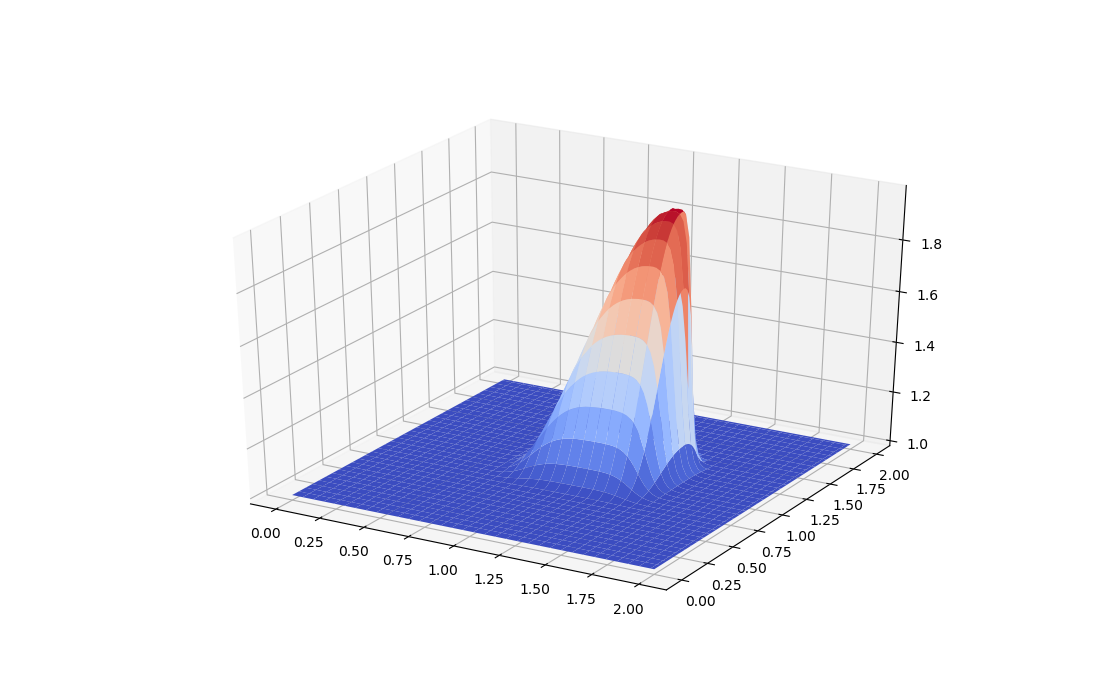
\includegraphics[width=1.8cm]{img/logo-neo.png}
\vspace*{0.35cm}\\
Instituto Navier Stokes -- INS \\

%\medskip
%\texttt{\{institutonavierstokes,ronety\}@gmail.com} % emails
}
\date{\today}

\AtBeginSection[]
{
\begin{frame}
\frametitle{Contenido}
\tableofcontents[currentsection]
\end{frame}
}

%%%%%%%% titulo e subtitulo %%%%%%%%
\title[Introducción a la modelación numérica]{Python Aplicado a la Fluidodinámica} 

%%%%%%%% nome dos autores %%%%%%%%
\author[Jhon, V. P.]{
Jhon Gesell Villanueva Portella} 

\begin{document}
\begin{frame}
\titlepage 

\end{frame}

\begin{frame}
\frametitle{Contenido} 
\tableofcontents 
\end{frame}

%%%%%%%% slides %%%%%%%%
\section{Introdución} 
\begin{frame}{Importancia de la Modelación numérica}
Al día de hoy no podemos negar que entender y saber de manera anticipada los eventos que van a ocurrir ayuda mucho al campo técnico en las ciencias e ingenierías y con el avance computacional que se ha desarrollado es importante que el profesional esté preparado para abordar a estos problemas, mediante herramientas de cálculo computacional el profesional puede reproducir o prevenir los acontecimientos en estudio, para nuestro curso este pretende dar las pautas iniciales para que el participante pueda orientar su camino en su formación, mostrando algunas de las fórmulas utilizadas en este estudio y también compartir código.
\end{frame}

\begin{frame}{Campos de aplicación}
\begin{itemize}
\item Análisis de resistencia de fallas mecánicas.
\item Polución de contaminantes en la atmósfera.
\item Comportamiento de las corrientes de viento en los alabes de los aerogeneradores.
\item Estudiar la capa límite en las ciudades a nivel regional.
\item Por ejemplo el flujo de sangre en un arteria.
\end{itemize}
\end{frame}


\begin{frame}{Python nuestro lenguaje de programación}
Python es un lenguaje interpretado y ello lo hace genial, tiene potencial para las las ciencias e ingenierías:
	\begin{itemize}
	\item Es un lenguaje multipropósito.
	\item Sintáxis clara y fácil de aprender.
	\item Programación orientada a objetos.
	\item Lo puedes usar como pegamento con otros lenguajes de 
	programación.
	\item Es open-source
	\item Multiplataforma para (Linux, Unix, WIndows y Mac Os).
	\end{itemize}
\end{frame}

\begin{frame}{Historia}
Python fue desarrollado en 1991 por el Holandez Guido van Roussun a finales de los años 80's, el nombre esta inspirado en el grupo humorista de la televisión Monty Python's Flying Circus, desde ese año al día de hoy ha evolucionado bastante, sobre todo ha desarrollado una comunidad realmente gigantezca, esa creo es su principal fortaleza, hay librerías para casi todo y sino lo puedes crear y tu mismo subir a la Internet, es muy demandado por las empresas.
\end{frame}



\section{Justificación}
\begin{frame}{Justificativa: blocos}
\begin{block}{Block 1}
Lorem ipsum dolor sit amet, consectetur adipiscing elit. Integer lectus nisl, ultricies in feugiat rutrum, porttitor sit amet augue. Aliquam ut tortor mauris. Sed volutpat ante purus, quis accumsan dolor.
\end{block}

\begin{block}{Block 2}
Pellentesque sed tellus purus. Class aptent taciti sociosqu ad litora torquent per conubia nostra, per inceptos himenaeos. Vestibulum quis magna at risus dictum tempor eu vitae velit.
\end{block}

\end{frame}

\section{Objetivos}
\begin{frame}{Objetivos}
\begin{block}{Objetivo Geral}
Presentar un curso que acerque al estudiante de la mecánica de fluidos a la modelación numérica.
\end{block}

\begin{block}{Objetivos Específicos}
\begin{itemize}
    \item Conocer las principales ecuaciones que gobiernan a los fluidos.
    \item Repaso general de ecuaciones diferenciales parciales.
    \item Método de diferencias finitas 1D
    \item Método de diferencias finitas 2D
	\item Método de diferencias finitas 3D
\end{itemize}
\end{block}

    
\end{frame}

\section{Fundamentos Teóricos}
\begin{frame}{Fundamentos Teóricos}
\begin{itemize}
    \item Ecucación de continuidad
    \item Ecucación de transporte
    \item Ecucación de cantidad de movimiento
\end{itemize}
    
\end{frame}

\begin{frame}{Fundamento teórico}
Nesta \textbf{abordagem} La mecánica de fluidos computacional es la ciencia que permite mediante el uso del ordenador reproducir fenomenos que ocurrieron o van a ocurrir para interés de las personas.
\medskip

\begin{itemize}
    \item Ríos, océanos y lagunas.
    \medskip
    \item Atmósfera.
\end{itemize}    
%\medskip

%\begin{teorema}[Masa  - energía equivalente ]
%$$E = mc^2$$
%\end{teorema}
\end{frame}

\begin{frame}{Pedazo de código}

Vamos a:
Repositorio/01/archivo01.py



\end{frame}

\section{Metodología}
\begin{frame}{Metodología}
\begin{columns}[c] % The "c" option specifies centered vertical alignment while the "t" option is used for top vertical alignment

\column{.45\textwidth} % Left column and width
\textbf{Pasos de la metodología}
\begin{enumerate}
\item Definir las ecucaciones
\item Discretizar las ecuaciones
\item Resolver las ecuaciones con el ordenador
\item Discutir los resultados
\end{enumerate}

\column{.5\textwidth} % Right column and width
Se sugiere que el público trate de discretizar las ecuaciones mediante diferencias finitas, responda en que casos aplicar diferencias finitas retrazadas, centradas o adelantadas.

\end{columns}
\end{frame}

\section{Resultados}
\begin{frame}{Resultados}
\begin{table}
\begin{tabular}{l l l}
\toprule
\textbf{Treatments} & \textbf{Response 1} & \textbf{Response 2}\\
\midrule
Treatment 1 & 0.0003262 & 0.562 \\
Treatment 2 & 0.0015681 & 0.910 \\
Treatment 3 & 0.0009271 & 0.296 \\
\bottomrule
\end{tabular}
\caption{Table caption}
\end{table}
\end{frame}

\begin{frame}{Resultados}
    
\begin{figure}
    \centering
    
\includegraphics[width=.7\textwidth]{img/river.jpg}
    \caption{Aqui temos a imagem de um lago}
    % \label{fig:my_label}
\end{figure}

\end{frame}

\section{Concluciones}
\begin{frame}{Conclusiones}
\begin{itemize}
\item La aplicación de la modelación numérica nos permite estudiar muchos campos aunque exige que las competencias de los profesionales aún sean mayores
\medskip
\item En Python todo es un objeto, lo importante es saber implementar los diferentes métodos que existen y ello se logra con una comprensión de las ecuaciones que  gobiernan los fenómenos, así como su discretización de estas.
\medskip
\item Los cuellos de botella se podrían reducir en caso se requiera con otros lenguajes como podría ser Fortran para ello se propone hacerlo con la librería F2PY.
\end{itemize}
    
\end{frame}


%%%%%%%% agradecimentos %%%%%%%%
\begin{frame}{Agradecimientos}
    \large{Agradecer al público interesado en el tema, a la directiva del Instituto Navier Stokes y al equipo organizador.}
\end{frame}
%------------------------------------------------


%------------------------------------------------
%------------------------------------------------
%%%%%%%% referencias %%%%%%%%
%\begin{frame}

%\nocite{*}
%\begin{frame}[allowframebreaks]{Referencias}
%\bibliographystyle{unsrt}
%\bibliography{ref.bib}
%\end{frame}


%%%%%%%% repite primer slide %%%%%%%%
\begin{frame}
\titlepage 
\end{frame}


\end{document}